\chapter{Auswirkungen}
\label{chapter:auswirkungen}


% cybercrime repräsentiert social engineering

\section{Prävalenz}

% wie ist die lage hinsichtlich der anzahl von angriffen
% surfshark globale ansicht
% repräsentativ für industrienationen: deutschland

\begin{figure}[!htp]
    \centering
    \begin{tikzpicture}

        \draw (0cm,0cm) -- (11cm,0cm);  %Abzisse
        \draw (0cm,0cm) -- (0cm,-0.1cm);  %linkes Ende der Abzisse
        \draw (11cm,0cm) -- (11cm,-0.1cm) node [rotate=60, below] {Jahr};  %rechtes Ende der Abzisse

        \draw (-0.1cm,0cm) -- (-0.1cm,5cm);  %Ordinate
        \draw (-0.1cm,0cm) -- (-0.2cm,0cm);  %unteres Ende der Ordinate
        \draw (-0.1cm,5cm) -- (-0.2cm,5cm) node [left] {Tsd.};  %oberes Ende der Ordinate

        \foreach \x [evaluate=\x as \i using int((\x + 0.0005) * 100 / 3)] in {0.3, 0.9,..., 4.8}  %Hilfslinien
            {
                \draw[gray!50, text=black] (-0.2cm,\x cm) -- (11cm,\x cm)
                node at (-0.5 cm,\x cm) {\small{\i}};
            };  %Beschriftung der Hilfslinien

        \foreach \i/\year [
            evaluate=\i as \y using (\i * 0.03),
            evaluate=\year as \x using ((\year-2007) * 0.6 + 0.5)
        ] in {
                34.2/2007,
                37.9/2008,
                50.3/2009,
                59.8/2010,
                59.5/2011,
                64.0/2012,
                64.4/2013,
                49.9/2014,
                45.8/2015,
                82.6/2016,
                86.0/2017,
                87.1/2018,
                100.5/2019,
                108.5/2020,
                124.1/2021,
                136.9/2022,
                134.4/2023
            }
            {
                \draw[fill=doc!60] (\x cm,0cm) rectangle (0.3cm+\x cm,\y cm) %die Säulen
                node at (0.2cm + \x cm,\y cm + 0.3cm) {\tiny{\i}}; %die Prozente über den Säulen
                \node[rotate=60, left] at (0.4cm +\x cm,-0.1cm) {\small{\year}}; %Säulenbeschriftung
            };

        \draw[red] (-0.1cm,0.7cm) -- (10.7cm,3.97cm); % fitting function: 6.062*(x)+23.3; 1 = year 2017 -> Tsd.


    \end{tikzpicture}
    \caption{Von der polizeilichen Kriminalstatistik (PKS) registrierte Straftaten im Bereich Cybercrime von den Jahren 2007 bis 2023. Zusammengetragene Werte aus den jährlich veröffentlichten Bundeslagebildern des Bundeskriminalamtes \bcite{pka}.
    Die in rot dargestellte Trendkurve wurde anhand der ungerundeten Werte kalkuliert und weist einen linearen Korrelationskoeffizienten von 0.9304 auf.}
    % Linear correlation coefficient
    % 0.9304
    % Coefficient of determination
    % 0.8656
    % Average relative error, %
    % 13.7771 %
\end{figure}
\FloatBarrier

\qq{Bei Cybercrime ist von einem sehr großen Dunkelfeld
auszugehen. Das heißt, dass vermutlich nur ein kleiner
Teil der Straftaten in diesem Bereich zur Anzeige
gebracht wird bzw. der Polizei und/oder den Strafverfol-
gungsbehörden bekannt ist.
Bereits 2013 hatte eine in Niedersachsen durchgeführte
Dunkelfeldstudie ein Dunkelfeld von 91 \% aller Cyber-
crimestraftaten errechnet04.} BKA

% demographische beurteilung (surfshark)

% (phishing bisher immer am verbeitestents)
% pretexting übernimmt phishing! warum? weil Business Email Compromise (BEC) unter phishing gewertet wird.
% es lohnt sich aber deshalb die psyhcologie zu betrachten
% Pretexting: 2022 (27\%), 2024 (more than 40\%)
% Phishing: 2022 ($\sim$ 70\%), 2024 (31\%)\cite{verizon2024,verizon2022}

% conversation hijacking wenig ,denn verlangt etwas erfolg bei vorherigen angriffen.
% z.b. folgt onversation hijacking oftmals auf account takeover.

% "Hackers are starting to increasingly use phishing as part of their
% ransomware attacks."\cite{3_barracuda}

% "Extortion attacks make up only 2\% of the total number of
% targeted phishing attacks we have seen in the past year. These
% attacks were mostly sextortion email threats, where hackers
% threaten to expose sensitive or embarrassing content to their
% victim’s contacts unless a ransom is paid. Demands are usually
% a few hundred or a few thousand dollars and need to be paid
% in bitcoin, which is difficult to trace. In the UK, the number of
% sextortion cases reported to National Crime Agency increased
% by 88\% between 2018 and 2020, and the number is expected to
% continue to increase"\cite{3_barracuda} stand 2021
% stand 2024: Extortion: ($\sim$ 25\%) \cite{verizon2024}
% Darunter fällt auch Ransomware

% "Account takeover is a form of identity theft and fraud where a
% malicious third party successfully gains access to a user’s account
% credentials"\cite{3_barracuda}
% "Account takeover is one of the fastest growing threats. In 2021,
% roughly 1 in 5 organizations (20\%) had at least one of their
% Microsoft 365 accounts compromised. This means that in 2021
% hackers managed to compromise around 500,000 Microsoft 365
% accounts around the globe."\cite{3_barracuda}


% warum immer mehr?
% Inzwischen hat sich die Gesamtzeit der Internetnutzung weltweit deutlich erhöht. Der durchschnittliche Internetnutzer verbringt nun fast sieben Stunden täglich online und das über
% alle Endgeräte hinweg. Das bedeutet, dass er mehr als zwei volle Tage einer Siebentagewoche im Internet unterwegs ist – im Vergleich zum Vorjahr ist hier ein Anstieg um 16
% Minuten oder vier Prozent zu verzeichnen. Der Report „Digital 2021“ zeigt, dass es im Januar 2021 weltweit 4,66 Milliarden Internet-User gab – ein Anstieg um 316 Millionen
% (7,3 Prozent) im Vergleich zum Januar 2020. -> mehr nutzer, mehr zeit im Internet

% &

% tools wie das social engineering toolkit https://github.com/trustedsec/social-engineer-toolkit machen angriffe immer simpler

% &

% und immer lukrativer (finanziell)


\section{Schaden}

Das finanzielle Motiv im Cybercrime ist nicht nur das primäre Motiv von Cyber Kriminellen, sondern verdrängt alle anderen Motive nahezu vollständig.
Neben einer finanziellen Motivation existieren beispielsweise Espionage und persönliche Motive, wobei Letztere statistisch außer Acht zu lassen sind.
Waren 2022 noch 11\% aller Data Breaches durch Espionage motiviert, so sind es 2023 gelegentlich 5\%.
Entsprechend stieg in diesen Jahren das finanzielle Motiv von 89\% auf 95\% an \bcite{verizon2022,verizon2024}.

Im Durchschnitt richtet ein 'Data Breach' 4.45 Millionen US-Dollar an Schaden an, wobei Social Engineering als initialer Angriffsvektor noch
über diesem Wert liegt \bcite{6_ibmsecurity}.
% https://cybersecurityventures.com/hackerpocalypse-cybercrime-report-2016/ TODO: 


Der Verlust, nach erfolgreichen Social Engineering Angriffen, ist jedoch für Unternehmen weitreichender.
Neben dem direkten finanziellen Verlust, durch den Diebstahl der Angreifer erleiden Unternehmen zusätzlich
Wiederherstellungskosten, da etwaige Daten verloren gegangen sind, und Sicherheitslücken gefunden und repariert
werden müssen. Des Weiteren entsteht eine Betriebsdisruption, was zu indirektem finanziellen Schaden, durch
Verlust von Produktivität, führt. Zuletzt erleiden Unternehmen einen Reputationsschaden, was in vielen Fällen
den verheerendsten Faktor ausmacht, insbesondere für kleinere Firmen \bcite{agony}.
Für Unternehmen können Cyber-Angriffe auch eine Form der Espionage darstellen, weshalb der Schaden eines
Unternehmens zusätzlich einen kompetitiven Schaden in der Marktwirtschaft darstellen kann. % hier auf lawyer page verweisen, evtl in bullet points

Individuen erleiden ebenfalls, neben finanziellen-, auch weitere Formen von Schäden.
Nicht außer Acht zu lassen ist der emotionale Schaden, da Personen oft, in Folge einer erfolgreichen
Manipulation, als naiv dargestellt werden. %bka
% Social Engineering MTTI (Mean Time To Identify): 218 Days
% Social Engineering MTTC (Mean Time To Contain) :  80 Days\cite{6_ibmsecurity}


% auch indiviuen können reputations schaden erleiden, siehe sextortion


% The median time for
% users to fall for phishing emails
% is less than 60 seconds. "\cite{verizon2024}


\begin{figure}[H]
    \centering
    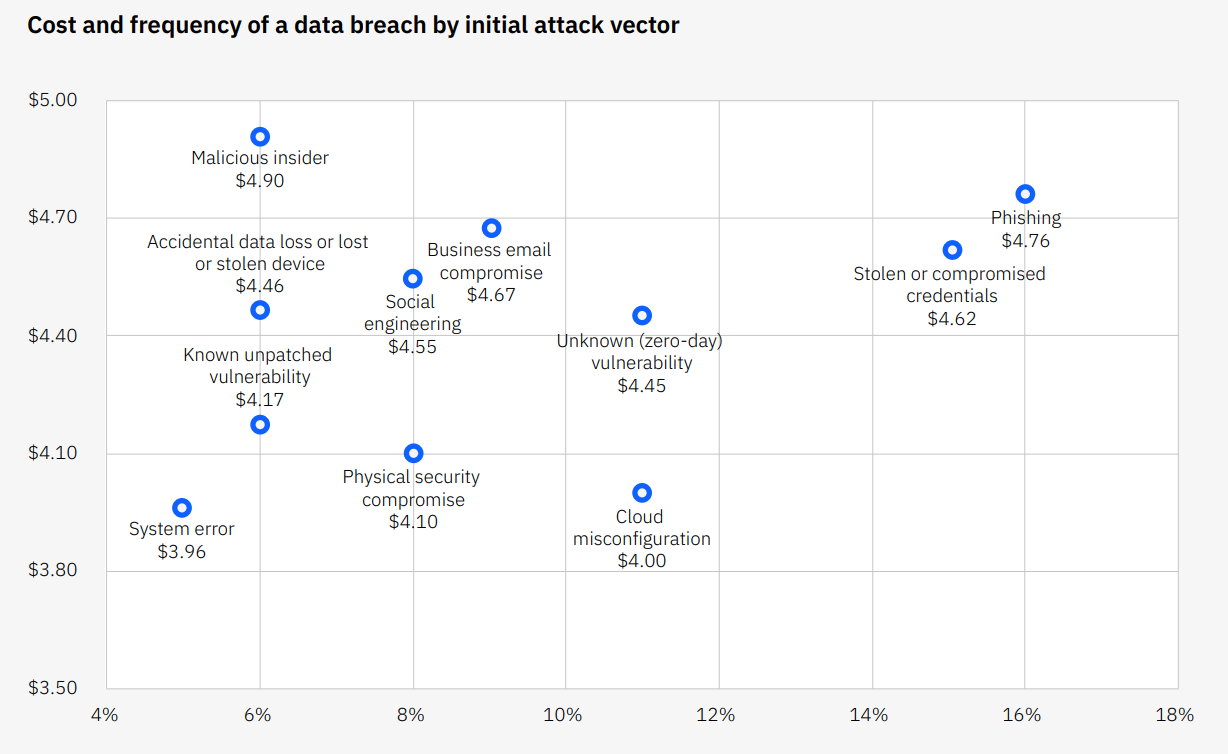
\includegraphics[width=5in]{IBM_Data.Breach.Report.png}
    \caption{IBM - Measured in USD millions}
\end{figure}
Avg. Kosten pro Breach (2022)


% \begin{figure}[H]
%     \centering
%     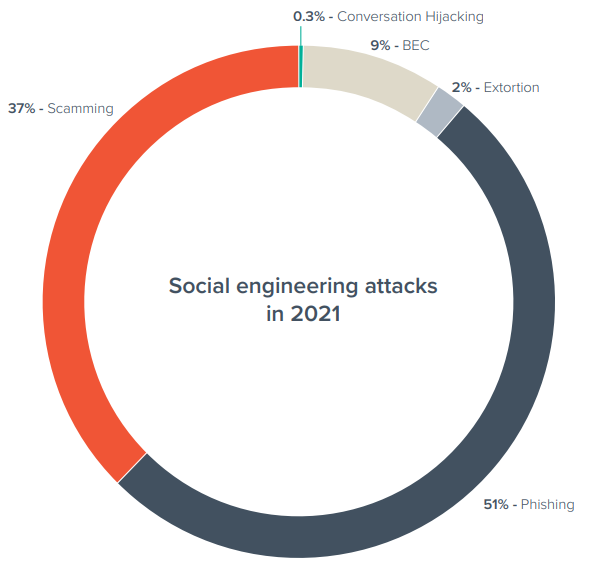
\includegraphics[scale=.5]{Barracuda_Social.Engineering.Attacks.png}
%     \caption{Barracuda - Social Engineering Attacks}
% \end{figure} % maybe ignore this


